\chapter{Missy mark, report selection and export contract}\label{ch:missy}

This chapter records the implemented option-3 mark, the report cover layout and the shared catalogue used by command, assisted, PDF and ZIP output.

\section{Selected mark}
The selected mark is option 3: hexagon, helix, MISSY, RUO and NOT VALIDATED. The warning text is present in full in compact and full forms. The mark is vector SVG and uses a deterministic font stack.

\begin{figure}[htbp]\centering
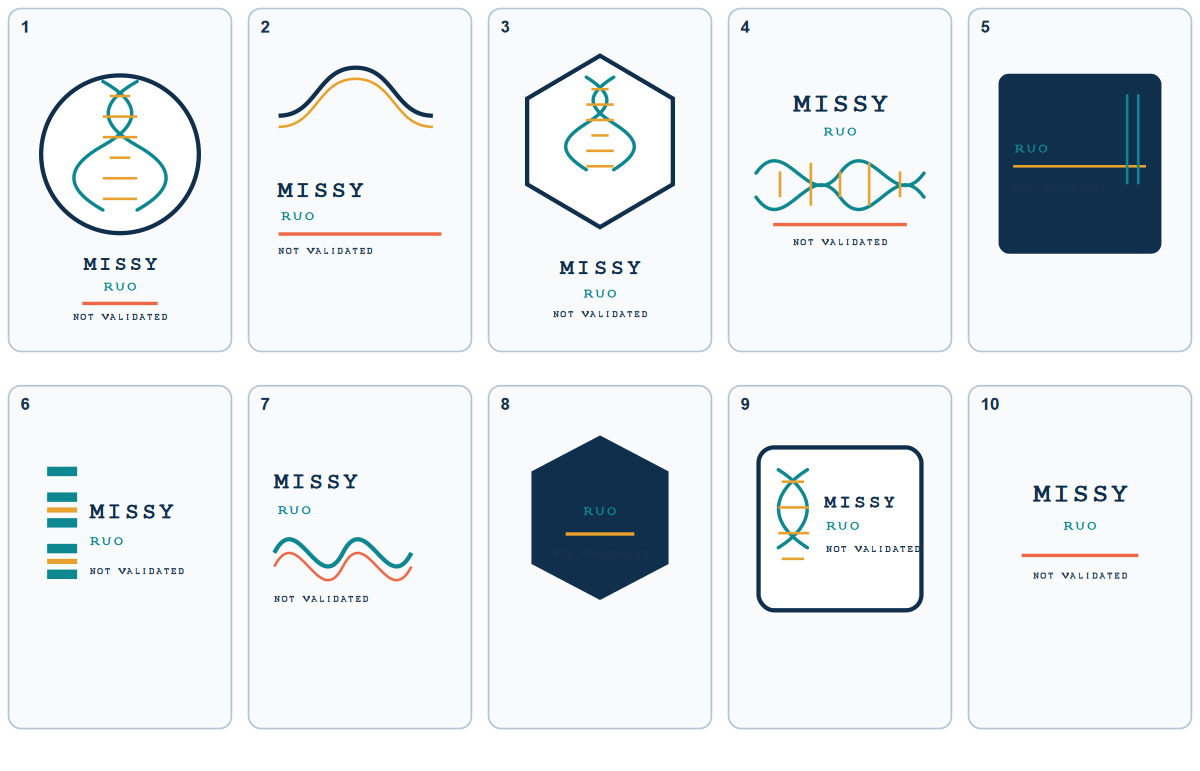
\includegraphics[width=0.96\textwidth]{fig/missy_logo_options.png}
\caption{Ten deterministic logo choices. Option 3 is used by the build.}\label{fig:missy-options}
\end{figure}

\begin{figure}[htbp]\centering

\includegraphics[height=5cm]{fig/missy_option3_full.png}
\caption{Selected option 3 mark.}\label{fig:missy-option3}
\end{figure}

\section{Report cover and footer}
Metadata values are wrapped to the report text width. A list of run names is one value per line; the PDF writer advances the cursor once per line. Every generated report page has a footer with the mark and the page count.

\begin{itemize}
  \item Stored Cq values and calls are not rewritten.
  \item Profile laboratory and analyst fields are included in the report metadata and profile hash.
  \item The footer reserves a 24 point lower band.
\end{itemize}

\section{Catalogue}
The current catalogue contains 25 graph figures, 18 data tables and 58 individual control-chart figures: 101 concrete items. The selectors \texttt{cc:all}, \texttt{cc:hardware}, \texttt{cc:software}, \texttt{cc:method} and \texttt{cc:operator} expand to the relevant chart items. The same item builders supply assisted mode, command mode, PDF and ZIP output.

\begin{longtable}{@{}p{3.1cm}p{4.0cm}p{7.0cm}@{}}
\toprule Identifier & Kind & Options \\\midrule\endfirsthead
\toprule Identifier & Kind & Options \\\midrule\endhead
\texttt{img:*} & figure & target, metric, signal, log, colourby, level, control \\
\texttt{data:*} & table & run, rows, pseudo \\
\texttt{rec:*} & table & run, rows, pseudo \\
\texttt{cc:*} & figure & type, x, phase1, lambda, L, k, h, specLo, specHi, warnAhead, charts \\
\bottomrule
\end{longtable}

\section{Command grammar}
\begin{itemize}
  \item \texttt{select pattern key=value}: validate all options, then add the selection.
  \item \texttt{set pattern key=value}: validate all options, then update selected items.
  \item \texttt{show pattern}: print options in force.
  \item \texttt{reset pattern}: remove options and use defaults.
  \item \texttt{cc:all} and group selectors expand without changing chart calculations.
\end{itemize}

\section{Implemented source}
The following listings are extracted from the production HTML snapshot. The black background is intentional for code readability; line numbers are HTML line numbers.

\vhead{Option-3 mark and SVG placement}
\lstinputlisting[firstnumber=11006,numbers=left,language=JavaScript]{code/missy_option3.js}

\vhead{Catalogue schema}
\lstinputlisting[firstnumber=11216,numbers=left,language=JavaScript]{code/missy_schema.js}

\vhead{Control-chart catalogue adapter}
\lstinputlisting[firstnumber=11270,numbers=left,language=JavaScript]{code/missy_chart_items.js}

\vhead{Option validation and command actions}
\lstinputlisting[firstnumber=11505,numbers=left,language=JavaScript]{code/missy_commands.js}

\vhead{Report cover and page generation}
\lstinputlisting[firstnumber=11424,numbers=left,language=JavaScript]{code/missy_report.js}

\begin{figure}[htbp]\centering

\includegraphics[width=0.96\textwidth]{fig/dna_separator.png}
\caption{DNA separator used between major document parts.}\label{fig:dna-separator}
\end{figure}


